\documentclass{article}
\usepackage[utf8]{inputenc}
\usepackage[spanish]{babel}
\usepackage{amssymb}
\usepackage{amsmath}

% Formato de página
\usepackage[letterpaper, margin = 1.5cm]{geometry}

% Más opciones para enumerar
\usepackage{enumitem}

% Manejo de imágenes
\usepackage{graphicx}
\usepackage{wrapfig}
\graphicspath{{img/}}
\usepackage{float}

\begin{document}
    \title{
        Fundamentos de bases de datos \\
        Tarea 5 \\
        Lenguaje de consulta SQL
    }
    \author{
        Díaz Gómez Silvia \\
        Eugenio Aceves Narciso Isaac \\
        Quiroz Castañeda Edgar
    }
    \date {
        13 de Mayo del 2019    
    }
    \maketitle
    Se tiene el siguiente esquema de bases de datos acerca de médicos, pacientes, ingresos consultas y
    especialidades:\\
    
   \begin{center}
   	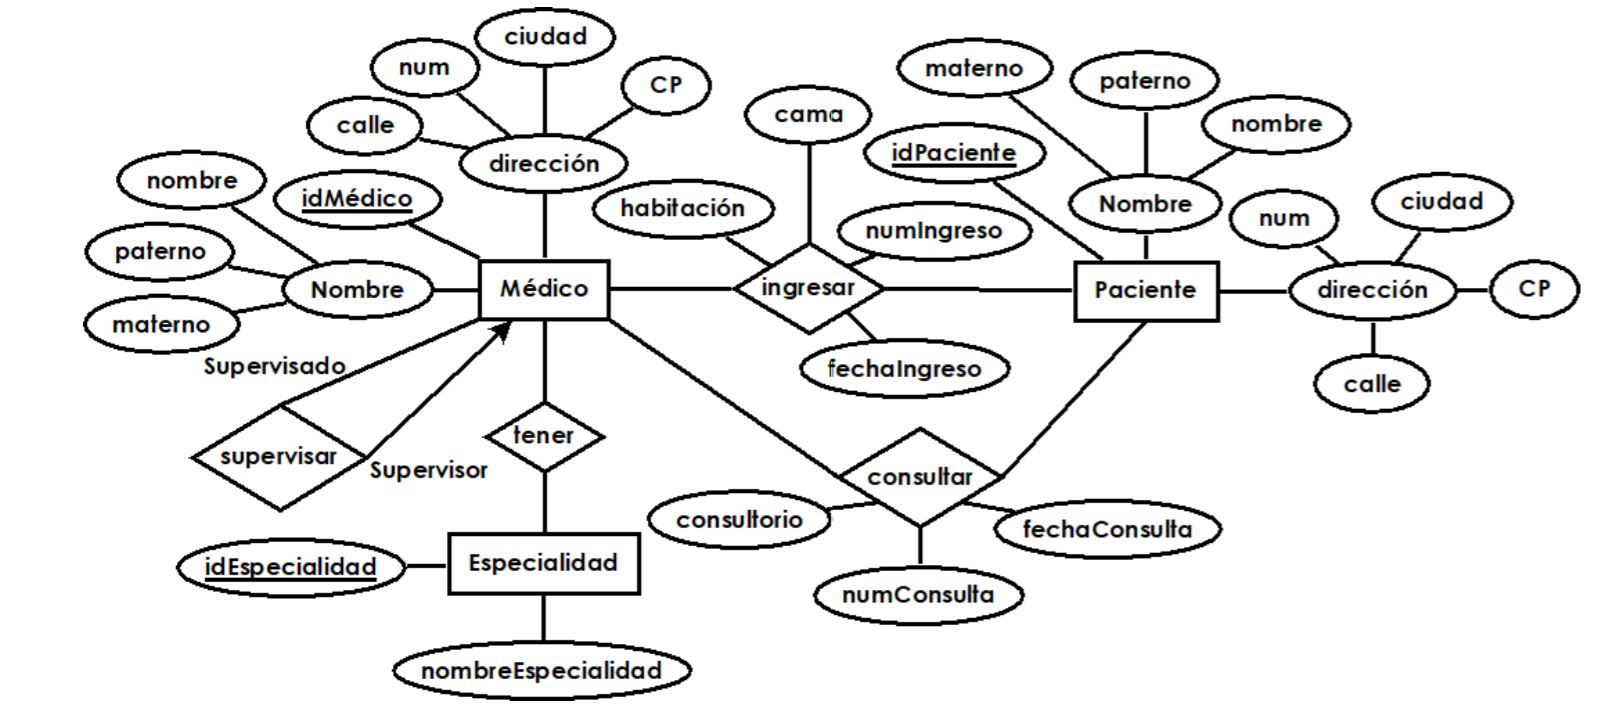
\includegraphics[width=1\textwidth]{img.JPG}
   \end{center}
    
    Resuelve los siguientes puntos:
    \begin{enumerate}
    	\item Traduce el modelo E-R a su correspondiente modelo relacional, indicando claramente las llaves
    	primarias y foráneas. No incluyas relaciones redundantes.\\
    	
    	\begin{center}
    		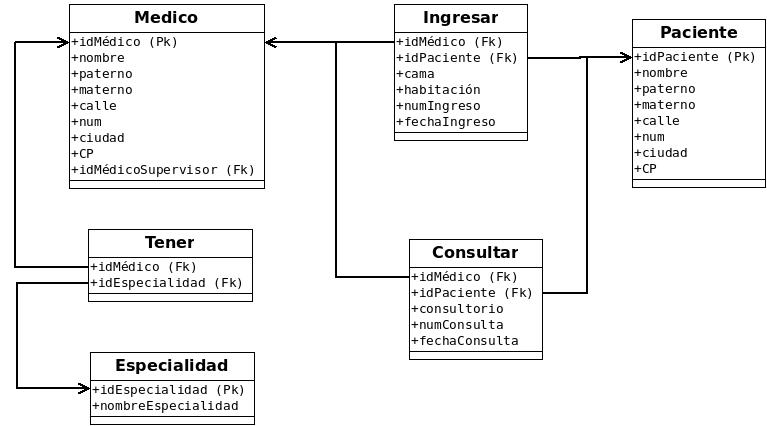
\includegraphics[width=1\textwidth]{DiagramaRelacional.jpeg}
    	\end{center}
        \item Proporciona un script en SQL que contenga el esquema de cada tabla incluyendo las restricciones
    	de integridad que consideres necesarias. Deberás incluir la totalidad de restricciones que se hayan
    	revisado en clase y/o en laboratorio y debe ser un esquema con Integridad Referencial; deberás
    	agregar alguna política de mantenimiento de FK. (ddl.sql)
    	
        \item Proporcionar un script en SQL que permita poblar el esquema anterior. (Mock\_data.sql)
        
        \item Consultas en sql (script dml.sql).
        
        En este inciso, se eliminó la consulta 'b' por involucrar información no contemplada en el diagrama
        (cumpleaños). Nos dimos cuenta de que la consulta 'q' tamién cae en esta categoría\footnote{No hay 
        modo de calcular la edad con los datos que se contemplan} y la eliminamos...
        
        Ah, también en la consulta 'p', que pide \textit{Total de pacientes que se han tenido por año y 
        especialidad en cada habitación \textbf{por tipo de cama}.} Supusimos que el tipo de cama esta dado
        por la habitación (Nuestras habitaciones son 'X-000' así que la letra X podría representearlo).
        
        \item Indica para la política de mantenimiento de llaves foráneas, qué ventajas y desventajas que tienen
        las políticas de establecimiento de nulos y cascada.
        
        \begin{itemize}
            \item Ventajas: Cascada refleja cambios de manera recursiva en todo lo afectado así que puede ahorrar
            mucho trabajo en comparación con todas las demás políticas de mantenimiento. Establecimiento de
            nulos resuleve de manera simple el problema de integridad y permite tener un ligero control sobre que 
            tuplas fueron afectadas (NULL podría ser como una etiquieta para algún caso, tipo una lista de pendientes).
            Como llaves foráneas entonces, cascada puede modificar todos los apuntadores y nulos mueve los apuntadores
            a un lugar donde estan 'seguros' y juntos.
            
            \item Des-ventajas: Con establecimiento de nulos puedes perder información de relaciones, lo cual 
            aunque preserva integridad, representa un inconveniente. Con cascada tus cambios pueden tener un 
            alcance muy grande y por tanto un alto potencial de 'daños' aunque se preserva la integridad. 
        \end{itemize}
        NOTA: En esencia, las obsevaciones aplican en ambos casos, DELETE y UPDATE.
        
   \end{enumerate}
\end{document}   
